\section{Згадки подій і два часові шари}
\label{sec:events}

Реконструкція подій приймає вже типізовані згадки, що містять присудок, ідентифікатори учасників та об'єктів, місце, посилання на докази й часові метадані. Вона не виділяє події автономно зі звітів, дописів чи відео. Ця межа відрізняє її від контрольованого виділення на основі фрагментів, де передбачені тригери й аргументи оцінюються за анотованим текстом \citep{wadden2019dygiepp}. Реалізований внесок --- консервативне впорядкування наданих тверджень.

Згадки комунікацій використовують час публікації; фізичні згадки потрапляють на свою часову шкалу лише за наданих найранішої й найпізнішої меж часу події. Відсутній або частково обмежений фізичний час зберігається без заміни часом публікації. Два шари показано на рисунку~\ref{fig:dual}. Попарні порівняння інтервалів дають відношення «раніше», «пізніше», «перекриття» або «невідомо», а кожне часове ребро явно позначене як непричинне. Упорядкування повідомлень не може встановити, що одна фізична дія спричинила іншу.

\begin{figure}[!htbp]
\centering
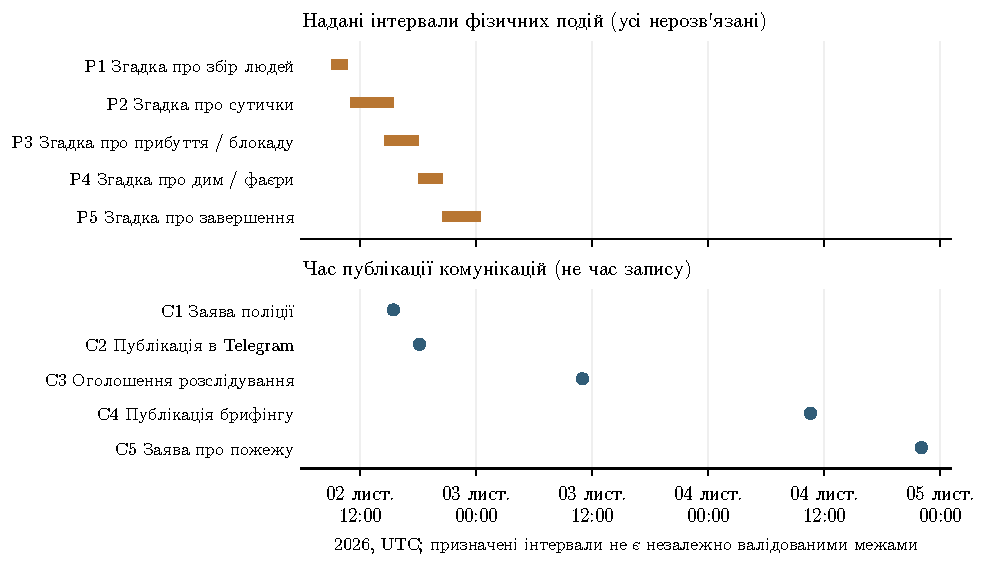
\includegraphics[width=\linewidth]{dual_timeline.pdf}
\caption{Окремі часові шкали комунікацій і фізичних подій. Час публікації визначає положення комунікацій; надані аналітиком інтервали --- положення повідомлених фізичних епізодів. Перекриття меж і нерозв'язані згадки лишаються видимими, а часовий порядок не має причинного тлумачення.}
\label{fig:dual}
\end{figure}

Точний збіг нормалізованого присудка, ідентифікаторів учасників і об'єктів та місця може створити придатний для перегляду зв'язок «можливо та сама подія» за умови часової сумісності й наданих заборон зв'язування. Функція ніколи не об'єднує згадки. Така стриманість важлива, бо подібні описи можуть стосуватися різних випадків подій; цю складність підкреслює ECB+ \citep{cybulska2014ecbplus}. Заборони зв'язування зберігають розрізнення, задані аналітиком; вони не є незалежно виявленими судженнями про тотожність.

Кураторська хронологія містить п'ять фізичних і п'ять комунікаційних згадок. Усі десять лишаються нерозв'язаними, зв'язків «можливо та сама подія» немає. Учасники, інтервали, позиції сторін і якісні рівні доказів задані в буквальному вхідному списку збирача. Ці рівні описують заявлену доказову основу, а не калібровану впевненість чи перевірене фізичне відбуття. Отже, артефакт демонструє відтворюване часове впорядкування та явну невизначеність; його підрахунки не вимірюють повноту виявлення подій чи точність реконструкції.
